\documentclass[11pt]{article}

\usepackage[margin=1in]{geometry}
\usepackage[T1]{fontenc}
\usepackage{lmodern}
\usepackage{microtype}
\usepackage{amsmath,amssymb}
\usepackage[dvipsnames]{xcolor}
\usepackage{enumitem}
\usepackage{needspace}
\usepackage[most]{tcolorbox}
\usepackage{tikz}
\usepackage[hidelinks]{hyperref}

\hypersetup{
  pdftitle={Homework 3 Solutions, MATH 327, Fall 2026},
  pdfauthor={Manish Patnaik},
  pdfsubject={MATH 327 homework problems}
}

\definecolor{courseblue}{HTML}{1F4E79}
\definecolor{lightblue}{HTML}{EAF2F8}
\definecolor{boxborder}{HTML}{B8CBDC}
\definecolor{darkgray}{HTML}{333333}

\setlength{\parindent}{0pt}
\setlength{\parskip}{0.55em}
\setlist[enumerate]{leftmargin=2em, itemsep=0.25em, topsep=0.3em}

\newtcolorbox{exercise}[2][]{
  enhanced,
  breakable,
  colback=white,
  colframe=boxborder,
  colbacktitle=lightblue,
  coltitle=courseblue,
  fonttitle=\bfseries,
  title={Exercise #2},
  title after break={Exercise #2 (continued)},
  boxrule=0.6pt,
  arc=1mm,
  left=2.5mm,
  right=2.5mm,
  top=1.5mm,
  bottom=1.5mm,
  before skip=0.8em,
  after skip=0.8em,
  #1
}

% Diagram modes: 1 = short diagonals, 2 = long diagonals, 3 = all.
\newcommand{\hexagondiagonals}[1]{%
  \begin{tikzpicture}[scale=0.85]
    \foreach \i in {1,...,6} {
      \pgfmathsetmacro{\vertexangle}{60*(\i-1)}
      \coordinate (v\i) at (\vertexangle:1.65);
      \node at (\vertexangle:2.05) {$v_{\i}$};
    }
    \draw[gray] (v1) -- (v2) -- (v3) -- (v4) -- (v5) -- (v6) -- cycle;
    \ifnum#1=2\relax\else
      \foreach \i in {1,...,6} {
        \pgfmathtruncatemacro{\j}{mod(\i+1,6)+1}
        \draw[thick,courseblue] (v\i) -- (v\j);
      }
    \fi
    \ifnum#1=1\relax\else
      \foreach \i in {1,...,3} {
        \pgfmathtruncatemacro{\j}{\i+3}
        \draw[thick,BurntOrange] (v\i) -- (v\j);
      }
    \fi
    \ifnum#1=2\relax\else
      \foreach \i in {1,...,6} {
        \pgfmathsetmacro{\labelangle}{60*\i}
        \node[fill=white,inner sep=1pt,font=\scriptsize,text=courseblue]
          at (\labelangle:0.825) {$d_{\i}$};
      }
    \fi
    \ifnum#1=1\relax\else
      \foreach \i in {1,...,3} {
        \pgfmathsetmacro{\labelangle}{60*(\i-1)}
        \node[fill=white,inner sep=1pt,font=\scriptsize,text=BurntOrange]
          at (\labelangle:1.2) {$\ell_{\i}$};
      }
    \fi
    \foreach \i in {1,...,6} {\fill (v\i) circle (2pt);}
  \end{tikzpicture}%
}

\newcommand{\chapterheading}[1]{%
  \par\vspace{0.5em}
  {\color{courseblue}\Large\bfseries #1}\par\vspace{0.35em}
  {\color{boxborder}\hrule height 0.6pt}\vspace{0.35em}
}

\newcommand{\sectionheading}[1]{%
  \Needspace{8\baselineskip}
  \vspace{0.25em}
  {\color{darkgray}\large\bfseries #1}\par
}


\definecolor{boxborder}{HTML}{B8CBDC}
\definecolor{darkgray}{HTML}{333333}
\definecolor{lightyellow}{HTML}{FFF9DC}
\definecolor{yellowborder}{HTML}{E4D58C}
\newtcolorbox{solution}{
  enhanced,
  breakable,
  colback=lightyellow,
  colframe=yellowborder,
  colbacktitle=lightyellow,
  coltitle=darkgray,
  fonttitle=\bfseries,
  title={Solution},
  title after break={Solution (continued)},
  boxrule=0.6pt,
  arc=1mm,
  left=2.5mm,
  right=2.5mm,
  top=1.5mm,
  bottom=1.5mm,
  before skip=0.2em,
  after skip=1em
}

\newcommand{\partlabel}[1]{\par\textbf{(#1)}\ }
\newcommand{\Z}{\mathbb Z}
\newcommand{\R}{\mathbb R}
\newcommand{\C}{\mathbb C}
\newcommand{\Stab}{\operatorname{Stab}}

\begin{document}

\begin{center}
  \colorbox{lightblue}{%
    \begin{minipage}{0.92\textwidth}
      \vspace{0.6em}
      \begin{tabular*}{\textwidth}{@{\extracolsep{\fill}}lr}
        {\color{courseblue}\bfseries\LARGE Homework 3} &
        {\color{courseblue}\bfseries\LARGE MATH 327}\\[0.4em]
        \multicolumn{2}{l}{\color{darkgray}\bfseries Fall 2026}\\[0.35em]
        \multicolumn{2}{l}{\color{courseblue}\bfseries Questions and solutions}\\[0.35em]
        \multicolumn{2}{l}{\color{darkgray}Covers Lectures 15--19}\\[0.2em]
        \multicolumn{2}{l}{\color{darkgray}Suggested completion date: Monday, October 26}
      \end{tabular*}
      \vspace{0.5em}
    \end{minipage}}
\end{center}

\vspace{0.5em}

Unless otherwise indicated, the following exercises are from Michael Artin's
\emph{Algebra}, second edition.

% Solutions adapted from the instructor's 2025 Homework 2 solutions:
% Artin 2.10.5, 2.11.6, 2.11.9, 2.12.4 and 2.12.5.
% S.1 adapts the conjugacy argument in the instructor's 2025 Homework 3 solutions.
% Supplementary dihedral solutions use this term's vertex labels.
\chapterheading{Chapter 2: Groups}

\sectionheading{Section 10: The Correspondence Theorem}

\begin{exercise}{10.5 (Adapted)}
Let $\varphi\colon S_4\to S_3$ be the homomorphism described in
Example 2.5.13. In class we determined the subgroups
\[
  A=\varphi^{-1}\bigl(\langle(123)\rangle\bigr)
  \qquad\text{and}\qquad
  H_1=\varphi^{-1}\bigl(\langle(13)\rangle\bigr).
\]
Perform a similar analysis to determine the subgroup
\[
  H_2=\varphi^{-1}\bigl(\langle(12)\rangle\bigr).
\]
\textit{Hint.} Relabel the vertices of the square as shown below and
consider its geometric symmetries as permutations in $S_4$.
\begin{center}
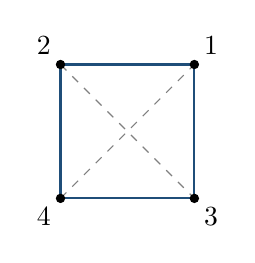
\begin{tikzpicture}[scale=0.85]
  \draw[thick,courseblue] (0,0) -- (2,0) -- (2,2) -- (0,2) -- cycle;
  \draw[dashed,gray] (0,0) -- (2,2) (0,2) -- (2,0);
  \fill (2,2) circle (2pt) node[above right] {$1$};
  \fill (0,2) circle (2pt) node[above left] {$2$};
  \fill (0,0) circle (2pt) node[below left] {$4$};
  \fill (2,0) circle (2pt) node[below right] {$3$};
\end{tikzpicture}
\end{center}
\end{exercise}

\begin{solution}
Use $\Pi_1=12\mid34$, $\Pi_2=13\mid24$, $\Pi_3=14\mid23$ and
\[
 V=\ker\varphi=\{1,(12)(34),(13)(24),(14)(23)\}.
\]
Let $r=(1243)$, the quarter-turn of the relabeled square, and $s=(23)$, reflection in the diagonal through vertices $1$ and $4$. Applying these permutations to the partitions gives
\[
 \varphi(r)=\varphi(s)=(12).
\]
Thus $L=\langle r,s\rangle\subseteq H_2=\varphi^{-1}(\langle(12)\rangle)$. We have $r^4=s^2=1$ and $srs=r^{-1}$, so the elements of $L$ are among $r^k,r^ks$ for $0\leq k<4$. These eight elements are distinct: the four powers of $r$ are distinct, and $s\notin\langle r\rangle$ (none of those powers is a transposition). Hence $|L|=8$ and $L\cong D_8$.

The correspondence theorem gives $|H_2|=|V|\,|\langle(12)\rangle|=8$. Since $L\subseteq H_2$, they are equal. Explicitly,
\[
 \boxed{H_2=\{1,(12)(34),(13)(24),(14)(23),(14),(23),(1243),(1342)\}.}
\]
Geometrically, these are exactly the symmetries of the square labeled $1,2,4,3$ around its boundary. The subgroup is not normal in $S_4$, since its image $\langle(12)\rangle$ is not normal in $S_3$.
\end{solution}

\begin{exercise}{S.1 (Supplementary)}
Prove that there is no surjective homomorphism $S_5\to S_4$.
\end{exercise}

\begin{solution}
Suppose $f:S_5\to S_4$ were surjective. Its kernel $K$ would be normal and would have order
\[
 |K|=\frac{120}{24}=5.
\]
Choose $1\ne a\in K$. Lagrange's theorem implies $a$ has order $5$, so as a permutation of five letters it is a $5$-cycle. Every $5$-cycle is conjugate to $a$: conjugation simply relabels its five entries. There are $5!/5=24$ such cycles. Normality would force all $24$ into $K$, contradicting $|K|=5$. Therefore no such surjection exists.
\end{solution}

\sectionheading{Dihedral Groups and Group Actions}

\begin{exercise}{1 (Supplementary)}
Let $n\geq3$. Define $D_{2n}$ by the presentation
\[
  D_{2n}=\langle x,y\mid x^n=1,\ y^2=1,\ yx=x^{n-1}y\rangle.
\]

\begin{enumerate}[label=\textbf{(\alph*)}]
	\item Prove that every element of $D_{2n}$ can be written uniquely in one of
	the forms
	\[
	x^k \qquad\text{or}\qquad x^k y,
	\qquad 0\leq k<n.
	\] 

	\item Let $H:=\{1,x,\ldots,x^{n-1}\}$. Show that $H$ is a normal subgroup of $D_{2n}$.

	\item Let $I:=\{1,y\}$. Is $I$ normal in $D_{2n}$? Justify your answer.


	\end{enumerate}


\end{exercise}

\begin{solution}
Recall $D_{2n}=\langle x,y\mid x^n=y^2=1,\ yx=x^{-1}y\rangle$.
\partlabel{a} The relation $yx=x^{-1}y$ moves every occurrence of $y$ to the right of every power of $x$. Using $y^2=1$ and reducing exponents modulo $n$, every word becomes $x^k$ or $x^ky$ with $0\leq k<n$. 
\partlabel{b} $H=\langle x\rangle$ is invariant under conjugation by $x$, and $yx^ky^{-1}=x^{-k}\in H$. Since $x,y$ generate the group, $H\trianglelefteq D_{2n}$. Equivalently, $H$ has index $2$.
\partlabel{c} $I=\{1,y\}$ is a subgroup of order $2$, but
\[
 xyx^{-1}=x^2y\ne y
\]
since $x$ has order $n\geq3$. Also $x^2y\ne1$ by uniqueness of normal forms. Thus $I$ is not normal.
\end{solution}

\begin{exercise}{2 (Supplementary)}
Let a group $G$ act on a set $S$. Recall that the \emph{orbit} of
$s\in S$ and its \emph{stabilizer} are defined by
\[
  O_s:=\{g\circ s\mid g\in G\},
  \qquad
  \operatorname{Stab}_G(s):=\{g\in G\mid g\circ s=s\}.
\]
Consider the natural action of $D_8$, the symmetry group of the square,
on its vertices $V=\{v_1,v_2,v_3,v_4\}$, labeled as follows.
\begin{center}
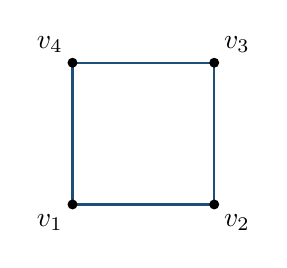
\begin{tikzpicture}[scale=0.9]
  \draw[thick,courseblue] (0,0) -- (2,0) -- (2,2) -- (0,2) -- cycle;
  \fill (0,0) circle (2pt) node[below left] {$v_1$};
  \fill (2,0) circle (2pt) node[below right] {$v_2$};
  \fill (2,2) circle (2pt) node[above right] {$v_3$};
  \fill (0,2) circle (2pt) node[above left] {$v_4$};
\end{tikzpicture}
\end{center}
Determine the orbit $O_{v_1}$ and the stabilizer
$\operatorname{Stab}_{D_8}(v_1)$.
\end{exercise}

\begin{solution}
Every vertex can be carried to $v_1$ by a rotation, so
\[
 O_{v_1}=\{v_1,v_2,v_3,v_4\}.
\]
The only symmetries fixing $v_1$ are the identity and reflection in the diagonal through $v_1$ and $v_3$. Therefore
\[
 \boxed{\Stab_{D_8}(v_1)=\{1,(v_2\ v_4)\}.}
\]
This also agrees with orbit--stabilizer: the stabilizer has size $8/4=2$.
\end{solution}

\Needspace{18\baselineskip}
\begin{exercise}[breakable]{3 (Supplementary)}
Consider the natural action of $D_{12}$ on the vertices
$V=\{v_1,\ldots,v_6\}$ of a regular hexagon, labeled counterclockwise
as shown below. Let $x$ be counterclockwise rotation through $\pi/3$,
and let $y$ be reflection across the diagonal joining $v_1$ and $v_4$.
\begin{center}
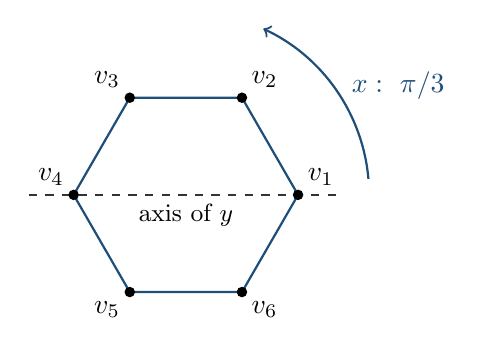
\begin{tikzpicture}[scale=0.95]
  \draw[thick,courseblue]
    (0:1.5) -- (60:1.5) -- (120:1.5) -- (180:1.5)
    -- (240:1.5) -- (300:1.5) -- cycle;
  \draw[dashed,thick,darkgray] (-2.1,0) -- (2.1,0);
  \node[below,font=\small] at (0,0) {axis of $y$};
  \fill (0:1.5) circle (2pt) node[above right] {$v_1$};
  \fill (60:1.5) circle (2pt) node[above right] {$v_2$};
  \fill (120:1.5) circle (2pt) node[above left] {$v_3$};
  \fill (180:1.5) circle (2pt) node[above left] {$v_4$};
  \fill (240:1.5) circle (2pt) node[below left] {$v_5$};
  \fill (300:1.5) circle (2pt) node[below right] {$v_6$};
  \draw[->,thick,courseblue] (5:2.45) arc (5:65:2.45);
  \node[right,text=courseblue] at (35:2.55) {$x:\ \pi/3$};
\end{tikzpicture}
\end{center}
\begin{enumerate}[label=\textbf{(\alph*)}]
  \item Describe geometrically each of the transformations
        $xy$, $x^2y$, $x^3y$, $x^4y$, and $x^5y$.
        Identify the axis of any reflection that occurs.
        Here products act from right to left, so $xy$ means first
        apply $y$, then $x$.
  \item Describe the homomorphism $\rho\colon D_{12}\to S_6$
        induced by this action by writing $\rho(x)$ and $\rho(y)$
        in cycle notation. Determine $\ker\rho$.
  \item \textbf{Short diagonals.}
        Let $\mathcal D_s=\{d_1,\ldots,d_6\}$, where
        $d_i=\overline{v_i v_{i+2}}$ and vertex subscripts are read
        modulo $6$.
        A diagonal is an unordered pair of endpoints, so a symmetry
        may preserve a diagonal while exchanging its endpoints.
        The short diagonals are shown in blue below.
        \begin{center}
          \hexagondiagonals{1}
        \end{center}
        Determine the orbits of $D_{12}$ on $\mathcal D_s$ and compute
        $\operatorname{Stab}_{D_{12}}(d_1)$.
        Describe the induced homomorphism
        $\rho_s\colon D_{12}\to S_6$ by giving $\rho_s(x)$ and
        $\rho_s(y)$ in cycle notation, using $d_i\leftrightarrow i$.
        Determine $\ker\rho_s$.
  \item \textbf{Long diagonals.}
        Let $\mathcal D_\ell=\{\ell_1,\ell_2,\ell_3\}$, where
        $\ell_i=\overline{v_i v_{i+3}}$.
        These diagonals join opposite vertices and are shown in orange.
        \begin{center}
          \hexagondiagonals{2}
        \end{center}
        Determine the orbits of $D_{12}$ on $\mathcal D_\ell$ and
        compute $\operatorname{Stab}_{D_{12}}(\ell_1)$.
        Describe the induced homomorphism
        $\rho_\ell\colon D_{12}\to S_3$ by giving $\rho_\ell(x)$ and
        $\rho_\ell(y)$ in cycle notation, using $\ell_i\leftrightarrow i$.
        Determine $\ker\rho_\ell$.
  \item \textbf{All diagonals.}
        Let $\mathcal D=\mathcal D_s\cup\mathcal D_\ell$ be the set of
        all nine diagonals, shown below.
        \begin{center}
          \hexagondiagonals{3}
        \end{center}
        Determine the orbits of $D_{12}$ on $\mathcal D$ and compute
        the stabilizer of a representative from each orbit.
        Describe the induced homomorphism
        $\rho_{\mathcal D}\colon D_{12}\to S_9$ by giving the images
        of $x$ and $y$ in cycle notation, using
        \[
          (d_1,d_2,d_3,d_4,d_5,d_6,\ell_1,\ell_2,\ell_3)
          \longleftrightarrow (1,2,3,4,5,6,7,8,9).
        \]
        Determine $\ker\rho_{\mathcal D}$.
\end{enumerate}
\end{exercise}

\begin{solution}
Number the vertices counterclockwise. In coordinates $t=i-1\in\Z/6\Z$ for $v_i$, the generators act by $x(t)=t+1$ and $y(t)=-t$.
\partlabel{a} The transformation $x^ky$ is reflection in the line through the center at angle $k\pi/6$ from the $v_1v_4$ axis. Indeed, on angles it sends $\theta$ to $k\pi/3-\theta$. Its axes are:
\begin{center}
\begin{tabular}{c|l}
Element & Reflection axis\\ \hline
$xy$ & Midpoints of $v_1v_2$ and $v_4v_5$\\
$x^2y$ & Vertices $v_2,v_5$\\
$x^3y$ & Midpoints of $v_2v_3$ and $v_5v_6$\\
$x^4y$ & Vertices $v_3,v_6$\\
$x^5y$ & Midpoints of $v_3v_4$ and $v_6v_1$
\end{tabular}
\end{center}
\partlabel{b} On the vertices,
\[
 \rho(x)=(123456),\qquad \rho(y)=(26)(35).
\]
The kernel is trivial: a rotation fixing every vertex is the identity, while a reflection fixes at most two vertices. Hence $\ker\rho=\{1\}$.
\partlabel{c} For the short diagonals $d_i=\overline{v_i v_{i+2}}$, rotation gives $x(d_i)=d_{i+1}$. Reflection sends $d_i$ to $d_{-i}$ (indices modulo $6$, so $d_0=d_6$). Consequently
\[
 \rho_s(x)=(123456),\qquad \rho_s(y)=(15)(24).
\]
There is one orbit, $\mathcal D_s$. Both $1$ and $x^2y$ preserve $d_1=\overline{v_1v_3}$, and orbit--stabilizer gives stabilizer size $12/6=2$. Thus
\[
 \Stab(d_1)=\{1,x^2y\}.
\]
The kernel lies in this stabilizer, but $x^2y$ sends $d_2$ to $d_6$. Hence $\ker\rho_s=\{1\}$.
\partlabel{d} On the long diagonals,
\[
 \rho_\ell(x)=(123),\qquad \rho_\ell(y)=(23).
\]
These generate $S_3$, and there is one orbit $\mathcal D_\ell$. Hence the kernel has order $12/6=2$. The half-turn $x^3$ preserves every long diagonal, so $\ker\rho_\ell=\{1,x^3\}$. The stabilizer of $\ell_1$ has order $12/3=4$ and is
\[
 \Stab(\ell_1)=\{1,x^3,y,x^3y\}.
\]
\partlabel{e} Length is preserved, and each of the short and long diagonal sets is transitive. Thus the two orbits are $\mathcal D_s$ and $\mathcal D_\ell$, with representative stabilizers as above. With the prescribed labels $1,\ldots,9$,
\[
 \rho_{\mathcal D}(x)=(123456)(789),\qquad
 \rho_{\mathcal D}(y)=(15)(24)(89).
\]
The kernel is trivial, since an element fixing every diagonal fixes every short diagonal and $\ker\rho_s=\{1\}$.
\end{solution}

\sectionheading{Section 11: Product Groups}

\begin{exercise}{11.6}
Let $G$ be a group that contains normal subgroups of orders $3$ and $5$,
respectively. Prove that $G$ contains an element of order $15$.
\end{exercise}

\begin{solution}
Let $H,K\trianglelefteq G$ have orders $3$ and $5$. Both are cyclic, so choose generators $a\in H$ and $b\in K$. The subgroup $H\cap K$ has order dividing both $3$ and $5$, hence $H\cap K=\{1\}$.

Normality implies
\[
 aba^{-1}b^{-1}=(aba^{-1})b^{-1}\in K,
 \qquad
 aba^{-1}b^{-1}=a(ba^{-1}b^{-1})\in H.
\]
Thus the commutator is trivial, and $a,b$ commute. Certainly $(ab)^{15}=1$. Conversely, if $(ab)^m=1$, commutativity gives $a^m=b^{-m}\in H\cap K$. Therefore $a^m=b^m=1$, forcing $3\mid m$ and $5\mid m$, hence $15\mid m$. It follows that $\boxed{\operatorname{ord}(ab)=15}$.
\end{solution}

\begin{exercise}{11.9}
Let $H$ and $K$ be subgroups of a group $G$. Prove that the product set
$HK$ is a subgroup of $G$ if and only if $HK=KH$.
\end{exercise}

\begin{solution}
Suppose first that $HK=KH$. The identity belongs to $HK$. If $h,h'\in H$ and $k,k'\in K$, then $kh'\in KH=HK$, so write $kh'=h''k''$. Hence
\[
 (hk)(h'k')=hh''k''k'\in HK.
\]
Also $(hk)^{-1}=k^{-1}h^{-1}\in KH=HK$. Thus $HK$ is a subgroup.

Conversely, if $HK$ is a subgroup, its set of inverses is itself. Since inversion reverses the order of multiplication,
\[
 HK=(HK)^{-1}=K^{-1}H^{-1}=KH.
\]
This argument does not require either subgroup to be finite.
\end{solution}


\sectionheading{Section 12: Quotient Groups}

\begin{exercise}{12.4}
Let $H=\{\pm1,\pm i\}$ be the subgroup of $G=\mathbb{C}^{\times}$ of
fourth roots of unity. Describe the cosets of $H$ in $G$ explicitly.
Is $G/H$ isomorphic to $G$?
\end{exercise}

\begin{solution}
For $z\in\C^\times$,
\[
 \boxed{zH=\{z,-z,iz,-iz\}.}
\]
These are the four vertices of a square centered at the origin, obtained by successively rotating $z$ through $\pi/2$. Two nonzero complex numbers define the same coset exactly when their ratio is one of $1,-1,i,-i$.

Consider the homomorphism $f:\C^\times\to\C^\times$ defined by $f(z)=z^4$. It is surjective because every nonzero complex number has a fourth root, and its kernel is exactly $H$. The first isomorphism theorem gives
\[
 \boxed{\C^\times/H\cong\C^\times,\qquad zH\longmapsto z^4.}
\]
The displayed map is well defined because $(zh)^4=z^4$ for $h\in H$.
\end{solution}

\begin{exercise}{12.5}
Let $G$ be the group of upper triangular real matrices
$\begin{bmatrix}a&b\\0&d\end{bmatrix}$ with $a$ and $d$ different from
zero. For each of the following subsets, determine whether or not $S$ is
a subgroup, and whether or not $S$ is a normal subgroup. If $S$ is a
normal subgroup, identify the quotient group $G/S$.
\begin{enumerate}[label=\textbf{(\roman*)}]
  \item $S$ is the subset defined by $b=0$.
  \item $S$ is the subset defined by $d=1$.
  \item $S$ is the subset defined by $a=d$.
\end{enumerate}
\end{exercise}

\begin{solution}
Write $g=\begin{pmatrix}a&b\\0&d\end{pmatrix}$, with $a,d\ne0$. Multiplication and inversion in $G$ satisfy
\[
 \begin{pmatrix}a&b\\0&d\end{pmatrix}
 \begin{pmatrix}a'&b'\\0&d'\end{pmatrix}
 =\begin{pmatrix}aa'&ab'+bd'\\0&dd'\end{pmatrix},
 \qquad
 g^{-1}=\begin{pmatrix}a^{-1}&-b/(ad)\\0&d^{-1}\end{pmatrix}.
\]
\partlabel{i} The diagonal matrices ($b=0$) form a subgroup, since the identity, products, and inverses are diagonal. It is not normal: for $u=\begin{pmatrix}1&1\\0&1\end{pmatrix}$,
\[
 u\begin{pmatrix}1&0\\0&2\end{pmatrix}u^{-1}
 =\begin{pmatrix}1&1\\0&2\end{pmatrix},
\]
which is not diagonal. Thus the indicated cosets do not form a quotient group under coset multiplication.
\partlabel{ii} The map $f_d:G\to\R^\times$, $g\mapsto d$, is a homomorphism by the multiplication formula. It is onto, since $\operatorname{diag}(1,t)$ maps to any $t\ne0$. Its kernel is exactly the subset $d=1$. Thus this subset is a normal subgroup and
\[
 \boxed{G/S\cong\R^\times,\qquad gS\longmapsto d.}
\]
\partlabel{iii} Similarly, $f_{a/d}:G\to\R^\times$, $g\mapsto a/d$, is a homomorphism, since the diagonal entries multiply separately. It is onto, using $\operatorname{diag}(t,1)$. Its kernel is exactly $a=d$. Consequently this subset is a normal subgroup and
\[
 \boxed{G/S\cong\R^\times,\qquad gS\longmapsto a/d.}
\]
\end{solution}

\vfill
{\small\color{darkgray}Compiled \today.}

\end{document}
